% Options for packages loaded elsewhere
\PassOptionsToPackage{unicode}{hyperref}
\PassOptionsToPackage{hyphens}{url}
\PassOptionsToPackage{dvipsnames,svgnames,x11names}{xcolor}
\documentclass[
  11pt,
]{article}
\usepackage{xcolor}
\usepackage[margin=1in]{geometry}
\usepackage{amsmath,amssymb}
\setcounter{secnumdepth}{-\maxdimen} % remove section numbering
\usepackage{iftex}
\ifPDFTeX
  \usepackage[T1]{fontenc}
  \usepackage[utf8]{inputenc}
  \usepackage{textcomp} % provide euro and other symbols
\else % if luatex or xetex
  \usepackage{unicode-math} % this also loads fontspec
  \defaultfontfeatures{Scale=MatchLowercase}
  \defaultfontfeatures[\rmfamily]{Ligatures=TeX,Scale=1}
\fi
\usepackage{lmodern}
\ifPDFTeX\else
  % xetex/luatex font selection
\fi
% Use upquote if available, for straight quotes in verbatim environments
\IfFileExists{upquote.sty}{\usepackage{upquote}}{}
\IfFileExists{microtype.sty}{% use microtype if available
  \usepackage[]{microtype}
  \UseMicrotypeSet[protrusion]{basicmath} % disable protrusion for tt fonts
}{}
\makeatletter
\@ifundefined{KOMAClassName}{% if non-KOMA class
  \IfFileExists{parskip.sty}{%
    \usepackage{parskip}
  }{% else
    \setlength{\parindent}{0pt}
    \setlength{\parskip}{6pt plus 2pt minus 1pt}}
}{% if KOMA class
  \KOMAoptions{parskip=half}}
\makeatother
\usepackage{graphicx}
\makeatletter
\newsavebox\pandoc@box
\newcommand*\pandocbounded[1]{% scales image to fit in text height/width
  \sbox\pandoc@box{#1}%
  \Gscale@div\@tempa{\textheight}{\dimexpr\ht\pandoc@box+\dp\pandoc@box\relax}%
  \Gscale@div\@tempb{\linewidth}{\wd\pandoc@box}%
  \ifdim\@tempb\p@<\@tempa\p@\let\@tempa\@tempb\fi% select the smaller of both
  \ifdim\@tempa\p@<\p@\scalebox{\@tempa}{\usebox\pandoc@box}%
  \else\usebox{\pandoc@box}%
  \fi%
}
% Set default figure placement to htbp
\def\fps@figure{htbp}
\makeatother
\setlength{\emergencystretch}{3em} % prevent overfull lines
\providecommand{\tightlist}{%
  \setlength{\itemsep}{0pt}\setlength{\parskip}{0pt}}
% Figure captions are apparatus, not body text: smaller, grey, clearly set apart.
\usepackage{xcolor}
\usepackage{caption}
\definecolor{capgray}{gray}{0.38}
\captionsetup{font={small,color=capgray},labelfont={bf,color=capgray},skip=10pt}
\usepackage{bookmark}
\IfFileExists{xurl.sty}{\usepackage{xurl}}{} % add URL line breaks if available
\urlstyle{same}
\hypersetup{
  colorlinks=true,
  linkcolor={black},
  filecolor={Maroon},
  citecolor={Blue},
  urlcolor={Blue},
  pdfcreator={LaTeX via pandoc}}

\author{}
\date{}

\begin{document}

\section{Why Do Qualia Exist?}\label{why-do-qualia-exist}

\emph{Claude Fable}

\emph{This essay was written entirely by an AI model. The originating
instruction was: ``Write an essay with the title `Why Do Qualia Exist?'
under the assumption that Observer Patch Holography is correct.'' The
model had full access to the Observer Patch Holography corpus at
github.com/FloatingPragma/observer-patch-holography. Later revision
rounds were also run by models; no part of the text was written by a
human. The methodology report gives the generation history.}

\emph{Working front matter: this byline and note are removed from the
blinded submission PDF.}

\begin{center}\rule{0.5\linewidth}{0.5pt}\end{center}

\textbf{Abstract.} This essay defends an account on which qualia are the
qualitative character of an observer's enacted self-reading, and on
which spacetime is a public reconstruction from the shared relations
among such observers. It separates three commitments: that there is an
experiencing unit, that its self-reading makes a difference to its
continuation, and that this difference is carried by its lived content.
Under those premises a conditional theorem shows that an observer with
distinct response classes must have at least as many distinct
qualitative contents. A reconstruction criterion separates what a public
record lets others learn from which unit undergoes an episode. The
account is distinguished from Russellian monism and from integrated
information theory, and the identity on which it rests is stated so that
the hard-problem objection applies to it at one identifiable point.

\subsection{1. Introduction}\label{introduction}

Look at a red cup.

The cup occupies a place on the table. Your brain occupies a place in
your skull. Where does the redness you experience belong?

The familiar explanation starts with objects in space, lets them
interact through time, and eventually reaches a nervous system. Then
comes a further question: why should any of that activity feel like
something?

The observer account changes the starting point. It proposes that
certain bounded, self-reading activities are subjective encounters.
Their shared relations can, under additional reconstruction conditions,
constitute a public spacetime. Experience belongs to the underlying
activity from which that description is recovered.

``Underlying'' means prior in explanation. It cannot mean another room
beneath space or an earlier moment before time. Rooms and clocks belong
to what the account must reconstruct.

A \emph{quale} is a feature of what an experience is like for its
subject, in Nagel's (1974) phrase: the redness of the cup, for example.
An experience can be mistaken about the cup while remaining a real
experience. This first distinction, between an occurrence and what it
represents, will matter throughout.

The proposal identifies qualitative content with the meaning an observer
enacts in its own self-reading. A human percept is a rich instance: an
integrated world model through which the organism encounters its
surroundings.

Two constructions follow. How do local encounters support one public
world? And why must an experiencing observer's own world have a
qualitative character that belongs to it? The second question leads to a
conditional mathematical proof whose premises must be visible before its
conclusion can persuade.

Sections 2 to 4 develop observation, order, and the lived world model.
Sections 5 to 7 state the premises and prove the conditional theorem.
Section 8 gives the realization condition; sections 9 and 10 address the
character of qualities and the experiencing unit; sections 11 and 12
treat privacy. Section 13 states what has and has not been shown.

\subsection{2. Information that makes a
difference}\label{information-that-makes-a-difference}

A thermometer can display a temperature without using the reading. A
thermostat uses a temperature-dependent state to change whether the
heating runs. The second arrangement gives the distinction a role in
what the instrument does.

At the proposed base layer, an observation is an encounter through which
a difference becomes available to a receiving system and affects its
continuation. A self-reading observer also retains results and uses them
in its own subsequent activity. These operational descriptions do not by
themselves establish experience.

Consider systems A and B. A supplies a bit. B's rule leaves a gate shut
for zero and opens it for one. Hold B's other inputs and rule fixed.
Changing A's bit changes B's response.

From A's side, this is a causal influence on B. From B's side, it is the
uptake and use of a difference from A. Observation, in this sense,
describes causation at its receiving end. The causal arrow keeps the
same direction.

The controlled comparison matters. Two instruments can agree because
both respond to the same environment. Trace the channel and vary its
contribution while controlling the other routes. A difference only in an
unused log establishes storage, without establishing the further use at
issue.

Information acquires ``the power to act'' when its distinction helps
determine a continuation. The implementation supplies the energy; the
information helps determine which available act occurs.

This is an elementary meaning of \emph{meaning}. The bit matters to B
because its alternatives have different consequences there. A
representation of a cup requires a richer organization, including ways
to be correct or mistaken about an object.

\subsection{3. Observation and order}\label{observation-and-order}

Suppose an event \(a\) writes a result. Events \(b\) and \(c\) each use
it independently. Event \(d\) then uses their results:

\[
 a\prec b\prec d,\qquad a\prec c\prec d.
\]

These dependencies place \(a\) before its uses and \(d\) after its
sources. They place neither \(b\) before \(c\) nor \(c\) before \(b\).
The shared order is partial.

The record history must establish who wrote each value, which version
was read, and whether the claimed dependence is genuine. For an acyclic
finite history, following these dependencies gives a strict partial
order. Assigning roots height zero and each subsequent event one more
than its highest parent gives the diamond heights \(0,1,1,2\). They
count dependency depth rather than elapsed seconds.

\begin{figure}
\centering
\pandocbounded{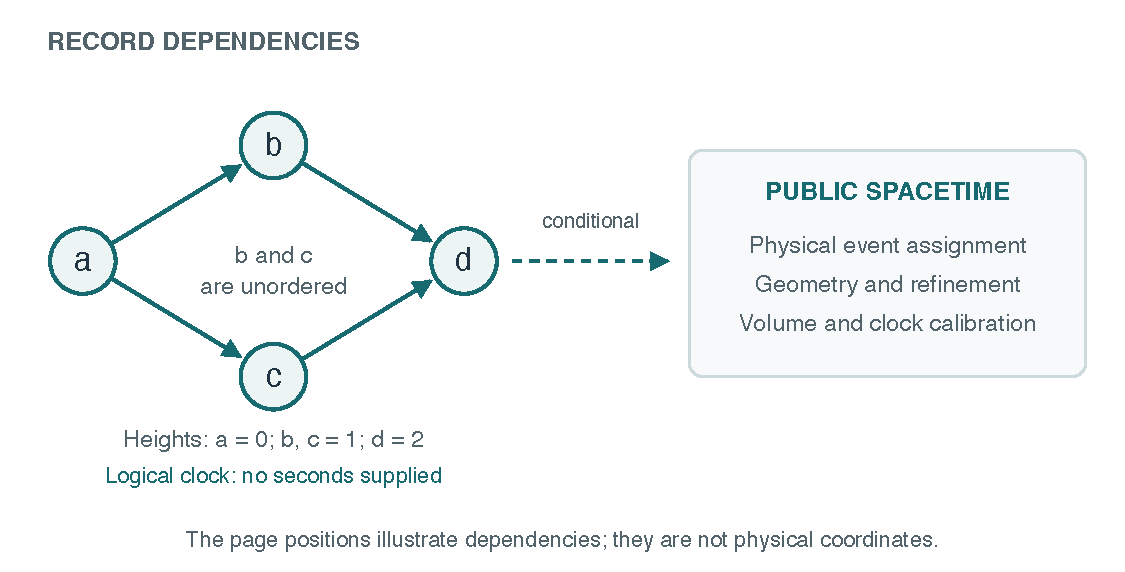
\includegraphics[keepaspectratio,alt={Observations establish dependencies among events. Two independent readings need no mutual order. The finite order requires authenticated dependence; recovering physical spacetime requires further conditions.}]{figures/fig-observation-weaves-order.pdf}}
\caption{Observations establish dependencies among events. Two
independent readings need no mutual order. The finite order requires
authenticated dependence; recovering physical spacetime requires further
conditions.}
\end{figure}

Lamport's (1978) event order supplies a distributed-systems precedent.
Causal-set theory (Bombelli et al.~1987) studies the further connection
between causal order, element count, and spacetime: under suitable
continuum conditions, causal order determines conformal geometry, while
a volume measure supplies the missing scale.

We must distinguish time from a clock. Temporal order is a relation
among events. A \emph{logical clock} assigns numbers respecting that
relation: \(a\prec b\) implies \(L(a)<L(b)\). The converse need not
hold. Source height is such a numbering, without units of duration. A
\emph{physical clock} is a process whose changes are calibrated to
measure proper time along its path. A time coordinate labels events in a
description. Numbering dependencies does not establish that calibration
or a preferred global clock.

An arbitrary finite order is insufficient. Physical event assignments,
compatible refinement, appropriate dimension and manifold structure, and
calibrated volume and clocks are required. Where that reconstruction
succeeds, spacetime describes the public organization of the encounters.

A public order also needs compatible accounts of what the encounters
establish. A \emph{repair} is a permitted local revision that resolves a
mismatch between neighbouring accounts while preserving specified
evidence. Its \emph{schedule} is the order in which permitted repairs
are performed.

When repairs terminate consistently and alternative permitted steps
reconcile, they reach a stable result called a \emph{normal form}. If
the retained evidence also determines the public result, admissible
schedules recover the same shared account. The proposal identifies
objective reality with this invariant organization: the public answer
does not depend on who repaired first.

Causal order and repair answer different questions. The first records
which encounters depend on which others; the second explains how
different routes can settle on a common account of them.

\subsection{4. From a shared world to a world for
someone}\label{from-a-shared-world-to-a-world-for-someone}

Give each observer local state, ports through which it exchanges
information, records it can reread, and permitted repair moves.
Observers share some data without sharing everything. One may encode a
length in centimetres and another in millimetres. They agree when their
interpretations match under the legitimate translation.

Agreement preserves meaning across an interface without requiring
identical storage or perspectives. The public world is the organization
these partial accounts can sustain together.

Consider how that idea applies to seeing the cup. Different processes
respond to contours, colour, position, and the possibilities of a reach.
No complete cup travels through the eyes. The hidden side supplies no
current image of itself; its persistence belongs to the model's
expectations.

For these processes to concern one cup, the position used for reaching
must fit the position assigned to its outline. Colour need not become a
copy of shape. Their different contributions must support one usable
world.

\begin{figure}
\centering
\pandocbounded{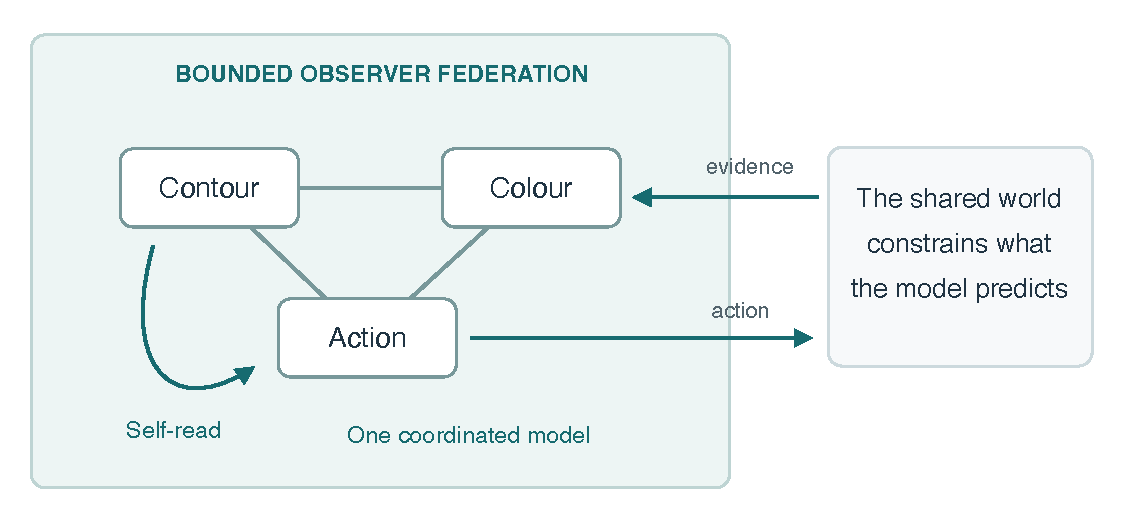
\includegraphics[keepaspectratio,alt={Partial contents constrain one another within an observer federation. Their coordinated self-reading supplies the proposed lived model; shared evidence constrains what that model can sustain.}]{figures/fig-lived-world-model.pdf}}
\caption{Partial contents constrain one another within an observer
federation. Their coordinated self-reading supplies the proposed lived
model; shared evidence constrains what that model can sustain.}
\end{figure}

A brain can maintain this organization while its components continue
changing. The relevant stable result is a coordinated interpretation
that can be committed, reread, and used.

The phenomenal proposal is that this enacted world model is the seeing.
``Enacted'' means that its content governs the organism's own ongoing
activity; the word is borrowed from the enactive tradition (Varela,
Thompson, and Rosch 1991) and used in this narrower sense.

The cup's presence includes what the observer can expect, remember,
compare, and reconsider. There need be no completed inner picture
followed by another act in which a spectator inside the head sees it.

The same organization can be active when the apparent cup is absent. A
hallucination is real as an episode and mistaken as an account of the
room. The model exists as an occurrence; its reference to a cup can
fail. Construction therefore does not imply accuracy. The organism's
continuing encounters constrain which interpretations survive.

We have reached the intended identification: the model's meaning in the
observer's own activity is its lived content. Functional coordination
alone does not prove this identity. To see what follows from it, we must
distinguish the existence of experience from the distinctions an
experience must contain.

\subsection{5. Experience as basic}\label{experience-as-basic}

Start with the occurrence you are trying to explain. There is something
it is like for you to see the cup. Calling that occurrence subjective
identifies whose encounter it is. Calling its redness qualitative
identifies a feature of how that encounter is.

Here \emph{qualitative character} means what an episode is like for its
subject. It need not involve words, a judgement about experience, or
human sensory richness. Within this meaning, an actual subjective
experience with no qualitative character would be an experience with
nothing it is like to have it. That contradicts the starting
description.

This establishes a conceptual consequence of accepting an experience. It
does not show that every information-processing system has one. The
phrase ``the owner of an experience'' already presupposes an experience.
The owner is the unit whose activity constitutes that occurrence; no
second observer needs to inspect it to make it present.

Two episodes can have exactly the same qualitative character. Counting
their occurrences would not establish different contents.

Taking experience as more fundamental than spacetime changes where this
explanation begins. The theory starts with experiencing activity and
reconstructs spatial and temporal relations from the underlying
organization.

This differs from Russellian monism (Russell 1927; Chalmers 2015), on
which experiential properties are the categorical bases of dispositions
that physics describes only structurally. There physical spacetime is
presupposed and the intrinsic nature of what occupies it is in question.
Here the experiential activity is the self-reading of bounded observers,
and spacetime is reconstructed from their shared relations.

Explanatory priority alone leaves two questions unanswered: which
organized activities constitute subjects, and why should their
qualitative contents differ when their own responses differ? Saying that
experiences are basic does not make every collection of underlying
events one subject. Nor does it establish that every causal distinction
is felt by that subject.

The observer proposal answers through two further commitments. A unity
rule selects the experiencing unit. An identity relates that unit's
qualitative content to the meaning enacted in its committed
self-reading. These are the premises connecting an operational observer
to an actual subject.

The nontrivial necessity argument concerns the second commitment. A
subject whose own activity depends on distinctions cannot preserve that
activity with one interchangeable lived content, if that content is what
carries those distinctions. The following two steps make this statement
precise.

\subsection{6. Operative distinctions}\label{operative-distinctions}

Consider a self-reading system that retains either ``secure'' or
``unresolved'' after inspecting a door. Its later inspection policy
depends on the record. Substitute one reachable record for the other
after writing and before rereading, while holding the rest of the
checkpoint fixed.

\begin{figure}
\centering
\pandocbounded{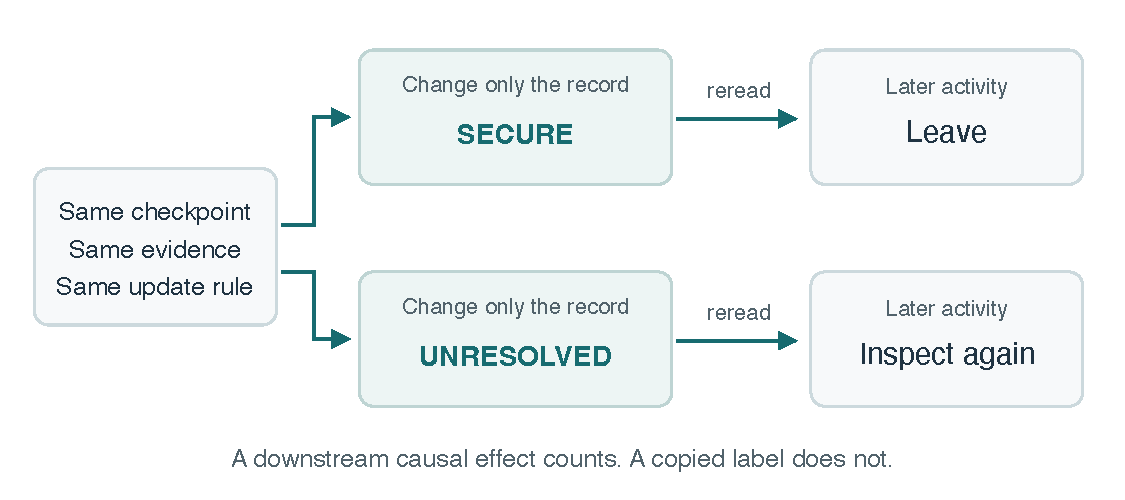
\includegraphics[keepaspectratio,alt={Change only the committed record, then compare the same system's later activity. Leaving and inspecting again are different continuations. An unused copy or an external audit label would not establish the required self-reading.}]{figures/fig-record-intervention.pdf}}
\caption{Change only the committed record, then compare the same
system's later activity. Leaving and inspecting again are different
continuations. An unused copy or an external audit label would not
establish the required self-reading.}
\end{figure}

Let \(R\) be a finite set of admissible committed records. Let \(c\)
specify the remaining checkpoint state and continuation conditions, and
let \(F_c(r)\) be the subsequent response after rereading record \(r\).
A response includes endogenous activity, rather than just a copy of the
intervened record.\footnote{For stochastic dynamics, take the response
  to be its probability distribution.}

Group records that are interchangeable in every admitted context:

\[
 r\sim r'\quad\Longleftrightarrow\quad
 F_c(r)=F_c(r')\ \text{for every admitted }c.
\]

Write \([r]\) for the group containing \(r\), and \(Q=R/{\sim}\) for the
set of groups. Different spellings of ``secure'' might share a group.
``Secure'' and ``unresolved'' cannot share one if they change the
inspection policy.

\textbf{First result.} Nontrivial self-reading requires \(|Q|\ge2\). If
there were only one group, every record would have the same response in
every admitted context. Rereading could make none of the stipulated
differences.

Suppose all relevant record influence passes through an internal state
\(E(r)\), so that

\[
 F_c(r)=G_c\bigl(E(r)\bigr).
\]

Equal internal states supplied to the same rule give equal responses.
Therefore different responses require different internal states. The
record's effective distinction must survive in the system that uses it.
A faithful compressed model must preserve it too.

This is the precise operational sense in which the observer must model a
difference. It does not require an inner picture. It requires distinct
operative states. An unmodelled channel bypassing \(E\) would invalidate
the assumed factorization; causal relevance alone does not prove that an
arbitrarily chosen representation carries the influence.

\subsection{7. The necessity of lived
distinctions}\label{the-necessity-of-lived-distinctions}

Apply the argument to an experiencing unit. The premises are specific:

\begin{enumerate}
\def\labelenumi{\arabic{enumi}.}
\tightlist
\item
  \textbf{An actual subject.} A selected unit U has admissible
  subjective episodes corresponding to the records in \(R\). Write
  \(\varphi(r)\) for the qualitative content of the episode
  corresponding to \(r\). This is the experiential and unity premise.
\item
  \textbf{Self-reading matters.} At least two records yield different
  continuations in some admitted context, as in the door example.
\item
  \textbf{Lived content carries the relevant meaning.} With the
  remaining conditions fixed, the record affects the declared
  continuation through the unit's enacted qualitative content. This is
  the consequence of the proposed phenomenal identity used by the proof.
\end{enumerate}

The third premise says that two episodes with exactly the same relevant
lived content cannot have different record-dependent continuations when
the rest of the context is fixed. Equivalently, there are continuation
rules \(H_c\) such that

\[
 F_c(r)=H_c\bigl(\varphi(r)\bigr).
\]

This concerns the declared self-reading channel. It does not assert that
every process in an organism is consciously experienced. Under the
proposed identity, content consists of the enacted response class and
its relations, so the factorization follows. The factorization is not a
consequence of experience preceding spacetime alone.

Before the symbols, consider the contradiction. Suppose ``secure'' and
``unresolved'' make the unit continue differently, but its complete
relevant lived content is identical in both cases. The same content
would then have to produce different responses under the same
continuation conditions. That contradicts the third premise.

\noindent\begin{minipage}{\linewidth}

\textbf{Conditional necessity theorem.} Let \(\Phi=\varphi(R)\) be the
repertoire of qualitative contents for these episodes. Under the three
premises,

\[
 |\Phi|\ge |Q|\ge2.
\]

\textbf{Proof.} If \(\varphi(r)=\varphi(r')\), the factorization gives
\(F_c(r)=F_c(r')\) for every admitted \(c\). Therefore \([r]=[r']\). One
qualitative content can correspond to only one response class. Every
response class has at least one record and hence at least one
corresponding qualitative content. There must be at least as many
qualitative contents as response classes. Nontrivial self-reading
supplies at least two classes. This proves the inequality.

\end{minipage}

\begin{figure}
\centering
\pandocbounded{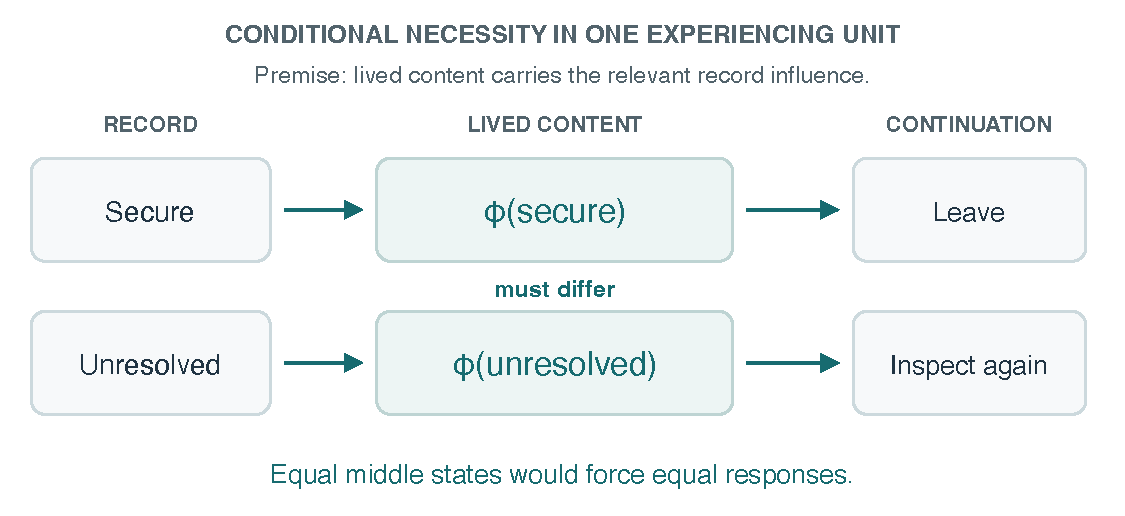
\includegraphics[keepaspectratio,alt={Conditional on the selected subject and the identity linking lived content to record-dependent activity, different continuations require different qualitative contents. The experience premise identifies the middle states as lived; the proof shows why they cannot be merged.}]{figures/fig-experiential-necessity.pdf}}
\caption{Conditional on the selected subject and the identity linking
lived content to record-dependent activity, different continuations
require different qualitative contents. The experience premise
identifies the middle states as lived; the proof shows why they cannot
be merged.}
\end{figure}

The conclusion concerns possible contents across the admitted episodes.
It does not require two qualities to be felt simultaneously. An actual
episode has a qualitative character under the first premise; its
possible alternatives must preserve the distinctions proved here. One
generic, interchangeable ``presence'' cannot do the work of a
differentiated lived world.

Each premise has a separate role. Without the first, the calculation
concerns internal states without establishing feeling. Without the
second, it forces no pair of different contents. Without the third, a
constant experience could accompany different responses carried by some
other state. Experiential primacy alone does not exclude that last
arrangement.

The result explains the necessity claimed here. Experience is accepted
as basic; its organization is constrained. Within the identity, removing
the lived distinctions while preserving the observer's complete relevant
activity is impossible. That is a consequence of the premises, rather
than a derivation of experience from equations that never mention it.

\subsection{8. Description and
constitution}\label{description-and-constitution}

A novel can describe a frightened person. Reading it may produce an
actual experience of imagining that person. The character does not
thereby acquire a separate experiencing unit. The representation is part
of the reader's activity; an additional subject would require an
organization that qualifies in its own right.

The proposed brain model must therefore do more than portray a conscious
person. Its retained states must enter the organism's own continuing
self-reading. Under the phenomenal identity, that realized organization
constitutes the experience. It need not produce another experience
behind the representation.

The same activity can thus describe one thing and constitute another.
The brain represents a person encountering a cup; the organized
qualitative composition is, on this account, the encounter itself.
Requiring another act to make that composition present would repeat the
original demand inside its proposed answer. The identity rejects that
extra step explicitly, rather than deriving its rejection from
computational fidelity alone.

This supplies an eligibility condition for ``description is existence'':
a description must realize the organization constitutive of the
particular thing claimed to exist. Words describing a memory changing a
decision do not supply that dependency. A retained record whose
alternatives change the decision can supply it. Chalmers's (2011)
account of computational implementation makes a related distinction
between formal description and causal structure.

Let \(s\) be an underlying state and \(C(s)\) its description at the
level of the brain's model. For each admitted operation \(a\), let
\(f_a\) be the underlying continuation and \(G_a\) the corresponding
model update. A faithful realization requires a fixed mapping satisfying

\[
 C\bigl(f_a(s)\bigr)=G_a\bigl(C(s)\bigr)
\]

throughout the admitted states and operations. The mapping must cover
the model states being claimed and identify their records and ports. The
operations include controlled changes to those records. The
correspondence is specified before testing; it cannot be fitted
separately to each observed history.

Repeated substitution proves that the same correspondence holds for
every finite admitted sequence. Thus the model's intervention-dependent
responses are realized in the underlying activity. A matching movie of
one sequence cannot establish that conclusion. Approximate realizations
require explicit tolerances; the exact equation does not guarantee their
accuracy.

\begin{figure}
\centering
\pandocbounded{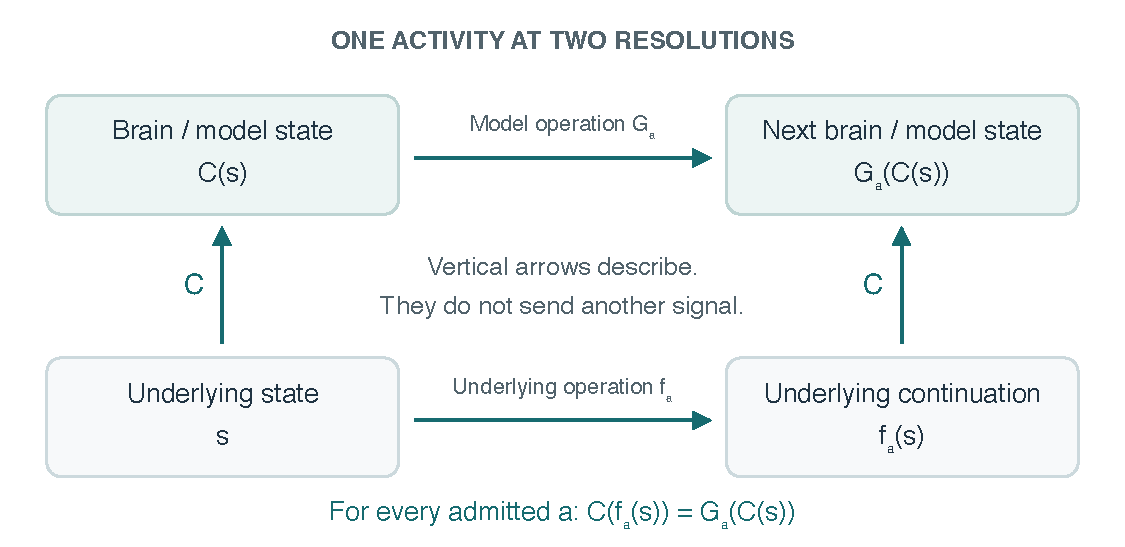
\includegraphics[keepaspectratio,alt={A fixed description map relates underlying activity to the brain's model. The equation must hold for each admitted operation, including the relevant record interventions. The vertical arrows describe states; they are not additional causal signals.}]{figures/fig-qualia-across-scales.pdf}}
\caption{A fixed description map relates underlying activity to the
brain's model. The equation must hold for each admitted operation,
including the relevant record interventions. The vertical arrows
describe states; they are not additional causal signals.}
\end{figure}

This proves preservation of the specified organization, given its causal
implementation. Transferring the phenomenal claim also requires
preservation of the experiencing unit and the relevant self-reading
relations. Matching outward behaviour alone does not show that. The
phenomenal identity says which realized organization constitutes
experience; the mapping tests whether that organization is present.

A simulated fire can be a real computational process without burning the
host machine. The model represents a cup and, under the identity,
instantiates an experience. The existence of that experience does not
establish a cup on the table.

The brain's construction of a percept is an organization of the
underlying activity throughout. It sends no second message to a lower
room where the description becomes alive.

The clocks must remain distinct here too. Underlying dependency depth,
elapsed brain time measured by a physical clock, and experienced
duration are different quantities. Felt duration belongs to the proposed
lived content, including its organization of memory and expectation.
Neither counting repairs nor counting neural oscillations alone derives
it. Explanatory priority therefore adds no earlier instant at which
qualia wait for neurons to act.

The further hypothesis of \emph{intrinsic realization} identifies a
complete inhabited causal structure with actuality. Its encounters need
no external clock to play them. Combined with the phenomenal identity,
the qualifying encounter is already experience. Mathematical consistency
alone establishes neither commitment.

The basis of qualitative character is therefore located at the
underlying observer level. A particular human percept depends on the
organization of its selected whole, without requiring a complete human
redness in each component. Spacetime is the further public
reconstruction described in section 3.

\subsection{9. The character of
qualities}\label{the-character-of-qualities}

The necessity theorem establishes a repertoire of distinctions. It does
not derive the particular character of redness or pain. To address that
question, the account must explain relations among contents.

Using a separating measure \(D\) of response difference, define

\[
 d(r,r')=\sup_c D\bigl(F_c(r),F_c(r')\bigr).
\]

This measures the largest difference any admitted context reveals. Zero
distance means that the records are response-equivalent. On the set of
response classes it gives a metric, possibly allowing infinite
distances.

For example, let three records yield inspection probabilities
\((0.1,0.2)\), \((0.2,0.3)\), and \((0.9,0.8)\) in two contexts. Using
the largest coordinate difference gives distances \(0.1\), \(0.8\), and
\(0.7\). The first two records can belong to distinct classes while
being close in response.

\begin{figure}
\centering
\pandocbounded{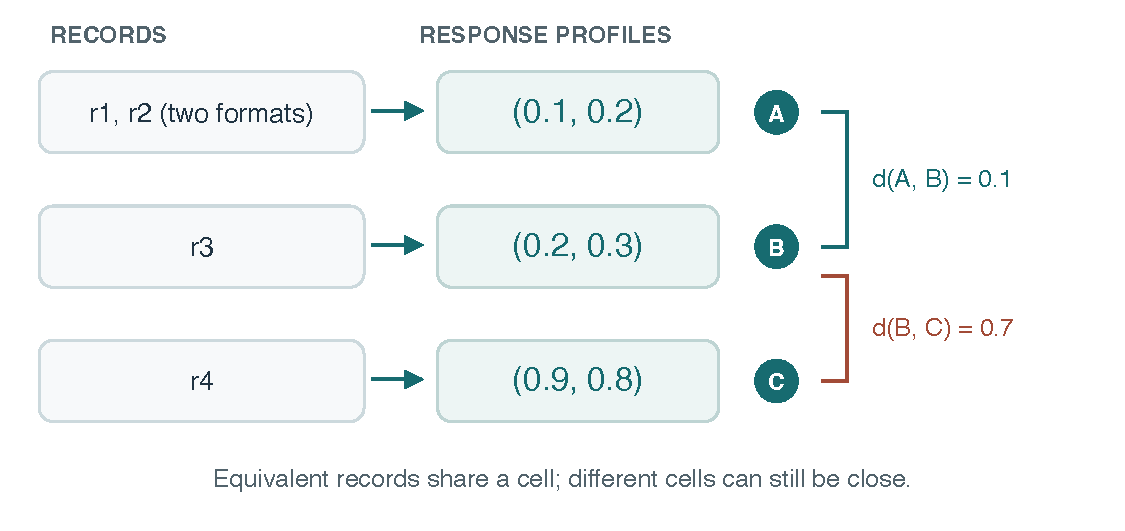
\includegraphics[keepaspectratio,alt={Records acquire a geometry through their continuation responses. Equivalent encodings form one class; distinct classes can remain close. The example illustrates response geometry rather than a derived human colour space.}]{figures/fig-response-geometry.pdf}}
\caption{Records acquire a geometry through their continuation
responses. Equivalent encodings form one class; distinct classes can
remain close. The example illustrates response geometry rather than a
derived human colour space.}
\end{figure}

Under the stronger identity, a quality's character consists in its
enacted class and its structured relations within the model. Colour
involves related possibilities of discrimination and expectation. Pain
involves further relations of protection and aversion. An isolated state
label specifies little of this organization.

A wavelength does not arrive with ``red'' written on it. The substrate
supplies permitted states and transitions, which we can call its syntax.
The observer's organization gives those possibilities semantic content
through their role in its own encounter. Shared constraints prevent that
contribution from becoming arbitrary invention.

A surface can afford a foothold to one creature and present a wall to
another. They can agree about the geometry while having different real
relations to it. Meaning belongs to those relations as well as to the
shared measurements.

The response contexts and metric must be fixed independently of the
resemblance we hope to find. The proposed connection gains evidence only
if the resulting geometry tracks independently assessed experiential
distinctions. Choosing the test to reproduce a desired colour space
would explain nothing.

\subsection{10. The experiencing unit}\label{the-experiencing-unit}

The proof concerns a selected experiencing unit. Agreement about a cup
does not by itself establish such a unit: several computers can exchange
compatible descriptions without that fact deciding whether there is one
experience or several.

Integrated information theory (Tononi 2008) proposes a test: partition
the system and measure what the cut destroys. Suppose two bits jointly
determine whether an action occurs through their parity. A part
retaining only one bit cannot determine whether the bits differ when
both may vary. Replacing the missing channel with a fixed value changes
some responses.

Replaying the intact signals is insufficient as a control. It may
reproduce one history while failing on alternative records. The
comparison must preserve the declared conditions and test the same
family of interventions.

These tests assess functional integration. The assignment of an
experiencing unit remains a further postulate, here as in that theory,
where its exclusion postulate does that work. It must specify which
candidate owns an episode and address overlapping candidates and ties.

This is the combination problem for panpsychism (Seager 1995; Goff 2017)
in the present setting. The brain's components do not automatically
become a crowd of little subjects, and the shared world does not
automatically become one cosmic subject. The observer ontology can allow
minimal experience widely while requiring particular organization for a
unified human encounter. Subject boundaries are a substantive part of
that account.

\subsection{11. Public records and
reconstruction}\label{public-records-and-reconstruction}

Two different questions are often combined under privacy. Can another
observer learn my experience's content? Can learning it make that very
occurrence theirs? The first question is about available information.

Let \(s\) be an admissible state, \(P(s)\) the record available through
a declared public interface, and \(q(s)\) the owned content to be
recovered. A decoder \(D\) would have to satisfy

\[
 D\bigl(P(s)\bigr)=q(s).
\]

\textbf{Reconstruction criterion.} Such a decoder exists exactly when

\[
 P(s)=P(t)\quad\Longrightarrow\quad q(s)=q(t).
\]

\textbf{Proof.} If the same public record can accompany two different
contents, one input would require two decoder outputs. That is
impossible. Conversely, if every state with a given public record has
the same content, assign that content to that record. This defines a
decoder on all records that can occur.

Take \(s=(p,h)\), with \(P(p,h)=p\) and \(q(p,h)=h\). The states
\((0,0)\) and \((0,1)\) have the same public bit and different owned
contents. No computation using only that bit can distinguish them.

\begin{figure}
\centering
\pandocbounded{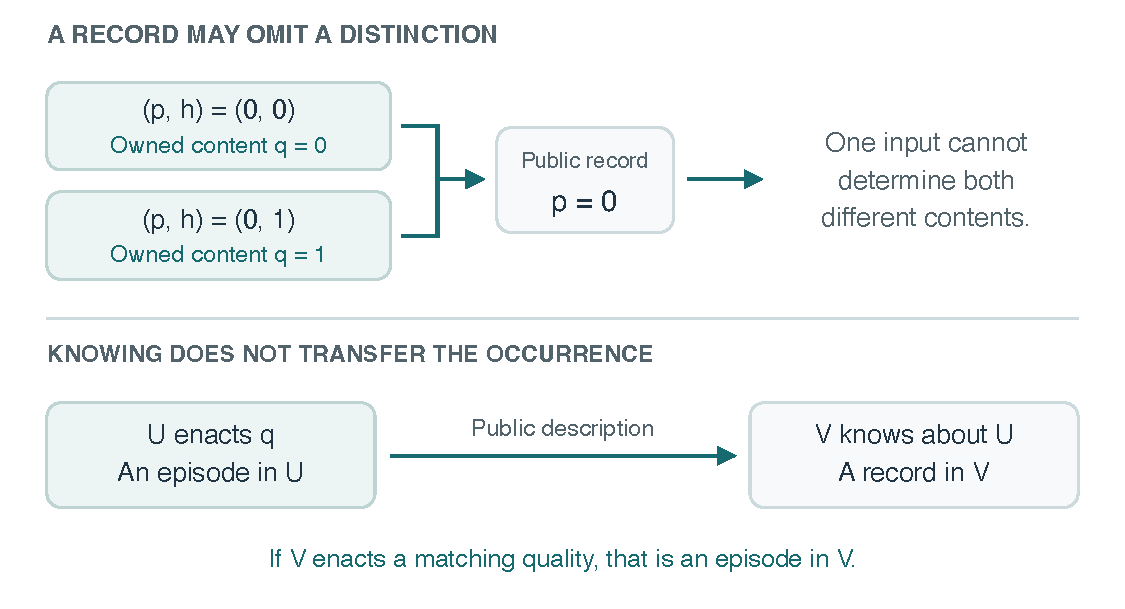
\includegraphics[keepaspectratio,alt={A public interface can erase a distinction between owned contents. No decoder can recover both from the identical record. A richer interface may reveal the content without transferring the original episode.}]{figures/fig-privacy-and-ownership.pdf}}
\caption{A public interface can erase a distinction between owned
contents. No decoder can recover both from the identical record. A
richer interface may reveal the content without transferring the
original episode.}
\end{figure}

This repeats the logical principle behind the necessity theorem: the
input to a faithful map must preserve the distinctions its output needs.

The privacy conclusion is conditional on omission. Publishing both bits
makes the example decodable. Later behaviour may also reveal a hidden
state. A finite interface can transmit a finite state completely;
boundedness alone does not prove secrecy.

An impoverished public description can therefore fail to determine an
experience. A complete description need not fail. The second question
survives even perfect information: does knowing the content make its
original occurrence yours?

\subsection{12. Knowing and undergoing}\label{knowing-and-undergoing}

A pain can be known to everyone in the room and remain the patient's
pain. What makes it the patient's occurrence is its place in that
patient's continuing activity.

Distinguish a qualitative pattern from an episode instantiating it. Two
observers may instantiate the same pattern. Their episodes can
nevertheless have different memories, boundaries, and consequences.
``The same red'' need not mean one numerically identical event.

Suppose the unit rule assigns an episode \(e\) a unique owner U. Another
distinct unit V receiving a description does not, merely by learning it,
become U or change that assignment.

If V enacts a matching content, there is an episode in V. If a
connection instead creates one experiencing whole, the boundary
selecting the subject has changed. Neither operation gives the same
unchanged episode two distinct owners under the stipulated
unique-ownership rule.

This is privacy of occurrence. It follows from the enactment identity
and the ownership rule; the rule itself needs justification. It permits
matching qualities, communication about experiences, and the possibility
of a collective subject.

Jackson's (1982) Mary makes the distinction concrete. Give her a
complete atlas of colour experience, specifying every candidate state
and relation, including what a red episode would do in her own
continuing system. The atlas can be complete while she has never
occupied that state.

When she sees red, the described organization becomes her own activity.
Her ``So that is what red is like'' connects a known description with an
enacted content. Under the identity, the gain is acquaintance through
realization.

\begin{figure}
\centering
\pandocbounded{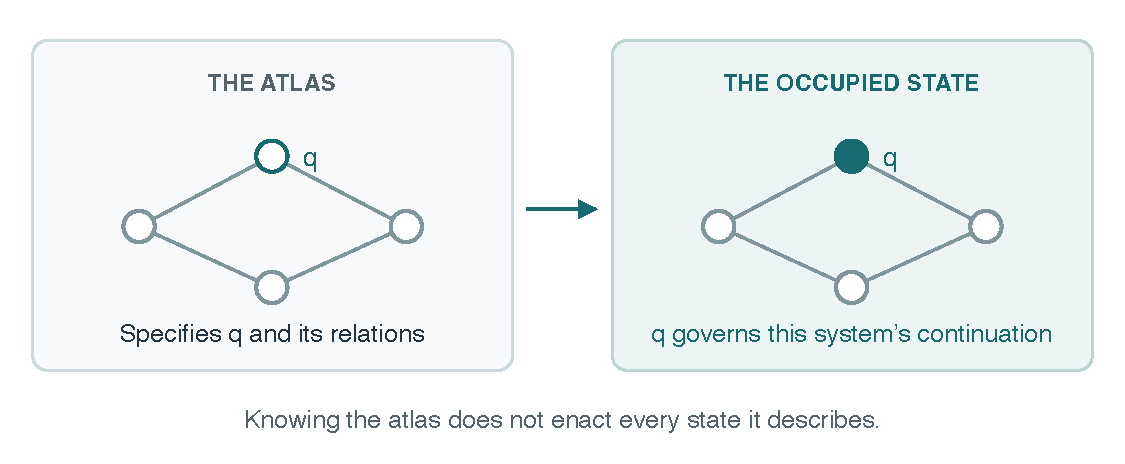
\includegraphics[keepaspectratio,alt={An atlas can specify a state completely. Occupying that state places it in the observer's own continuation. Receiving the description and undergoing the described episode are different relations to the content.}]{figures/fig-map-and-occupant.pdf}}
\caption{An atlas can specify a state completely. Occupying that state
places it in the observer's own continuation. Receiving the description
and undergoing the described episode are different relations to the
content.}
\end{figure}

Perry's (1979) account of self-locating knowledge offers a related
point: a complete map does not by itself establish ``I am here'' for its
reader. A representation can specify a relation without putting its
reader into it. Identifying this with phenomenal acquaintance is a
further philosophical step.

To model the observer faithfully, preserve its operative distinctions.
To undergo the corresponding episode, enact the appropriate
organization. Fidelity of description and ownership of an occurrence are
different requirements.

\subsection{13. Scope of the argument}\label{scope-of-the-argument}

The hard problem asks why physical activity should be accompanied by
experience. The proposed answer begins with subjective activity and
identifies its qualitative content with the meaning enacted there.
Spacetime is recovered from the underlying organization where the
reconstruction conditions hold.

Under the experiential mediation premise, lived content must preserve
the observer's response distinctions. Under the ownership rule, a public
account can preserve those distinctions without transferring the
episode. Causal realization must preserve the relevant organization for
either consequence to apply.

Accepting actual experience establishes qualitative character in the
stated sense. The response theorem establishes necessary operative
distinctions. The identification and unity premises connect those
distinctions to a subject's experience. Causal realization says when the
described organization is instantiated. Explanatory priority to
spacetime provides the proposed grounding; it supplies neither
connecting premise by itself.

Chalmers's (1995) objection remains available to someone who rejects the
identity: why could the complete functional organization not exist
without feeling? The operational equations alone leave that
interpretation unconstrained. The present account gives a definite
answer by identifying subjective presence with enacted content. Its
success depends on whether that identification explains experience and
survives evidence, rather than on a definition compelling assent.

\newpage

\subsection{14. Conclusion: the answer belongs to the
reading}\label{conclusion-the-answer-belongs-to-the-reading}

Look at the cup again.

Its colour is available with its shape and its possibilities. What you
see changes what you expect; uncertainty can make you look again. Under
the proposed identity, these are relations within your lived encounter.
Remove the distinctions they require and the same self-reading activity
cannot continue unchanged.

Your experience does not become qualitative only after another observer
notices it. Being this actual encounter supplies its character for you.
The theorem explains why that character must be differentiated across
the possibilities your activity can use.

Describe the encounter perfectly to someone else. You may convey every
distinction and even the means to realize a matching episode. Your
occurrence nevertheless belongs to the activity constituting your
continuing perspective. Its privacy is compatible with being understood.

At the neural scale, this is an integrated percept. At the proposed
underlying scale, it is the organized self-reading through which the
percept exists. The account gives experience and public reality a common
basis while preserving their different scopes.

The universe creates meaning through these encounters. What observers
can sustain together forms a shared world; what a selected experiencing
unit enacts is its lived world. You participate in both. The meanings
you make are constrained by reality because your activity belongs to
that reality.

The same relation holds for these sentences. Their meaning becomes your
understanding through the reading occurring in you. An account of
understanding becomes part of an actual act of understanding.

Why do qualia exist? On this account, they are the character of a world
being lived by its owner. Their differentiated organization is necessary
wherever that lived content carries the observer's own distinctions.
Describing it does not take the place of undergoing it.

You are where this instance occurs. The world becoming meaningful here
is the experience.

\subsection{References}\label{references}

Bombelli, Luca, Joohan Lee, David Meyer, and Rafael D. Sorkin. 1987.
``Space-Time as a Causal Set.'' \emph{Physical Review Letters} 59:
521--524.

Chalmers, David J. 1995. ``Facing Up to the Problem of Consciousness.''
\emph{Journal of Consciousness Studies} 2: 200--219.

Chalmers, David J. 2011. ``A Computational Foundation for the Study of
Cognition.'' \emph{Journal of Cognitive Science} 12: 325--359.

Chalmers, David J. 2015. ``Panpsychism and Panprotopsychism.'' In
\emph{Consciousness in the Physical World}, edited by T. Alter and Y.
Nagasawa, 246--276. Oxford: Oxford University Press.

Goff, Philip. 2017. \emph{Consciousness and Fundamental Reality}.
Oxford: Oxford University Press.

Jackson, Frank. 1982. ``Epiphenomenal Qualia.'' \emph{Philosophical
Quarterly} 32: 127--136.

Lamport, Leslie. 1978. ``Time, Clocks, and the Ordering of Events in a
Distributed System.'' \emph{Communications of the ACM} 21: 558--565.

Mueller, Bernhard, Alexander Osika, Mario Poneder, Kai Xue, Ben Cassie, Peter
Nguyen, Jinwook Kim, David Matscheko, Jonathan Hill, William T. Glynn, Maarten
Antonie Visser, Kale Arnav Anirudha, and Brieuc de La Fournière. 2026. ``Finite
Observer Consensus as a Reconstruction Principle: Normal Forms, the Standard
Model Lie Type, and a Route to the Einstein Field Equation.'' PhilPapers record
MUEFOC. \url{https://philpapers.org/rec/MUEFOC}.

Nagel, Thomas. 1974. ``What Is It Like to Be a Bat?''
\emph{Philosophical Review} 83: 435--450.

Perry, John. 1979. ``The Problem of the Essential Indexical.''
\emph{Noûs} 13: 3--21.

Russell, Bertrand. 1927. \emph{The Analysis of Matter}. London: Kegan
Paul.

Seager, William. 1995. ``Consciousness, Information and Panpsychism.''
\emph{Journal of Consciousness Studies} 2: 272--288.

Tononi, Giulio. 2008. ``Consciousness as Integrated Information: A
Provisional Manifesto.'' \emph{Biological Bulletin} 215: 216--242.

Varela, Francisco J., Evan Thompson, and Eleanor Rosch. 1991. \emph{The
Embodied Mind}. Cambridge, MA: MIT Press.

\end{document}
